\documentclass[11pt, oneside]{article}   	% use "amsart" instead of "article" for AMSLaTeX format
\usepackage{geometry}                		% See geometry.pdf to learn the layout options. There are lots.
\geometry{letterpaper}                   		% ... or a4paper or a5paper or ... 
%\geometry{landscape}                		% Activate for rotated page geometry
\usepackage[parfill]{parskip}    		% Activate to begin paragraphs with an empty line rather than an indent
\usepackage{graphicx}				% Use pdf, png, jpg, or eps§ with pdflatex; use eps in DVI mode
								% TeX will automatically convert eps --> pdf in pdflatex		
\usepackage{amssymb}
\usepackage{color}

%SetFonts

%SetFonts


\title{3 Month TAP Report}
\author{Helen Davies}
\date{}							% Activate to display a given date or no date

\begin{document}
\maketitle

\section{Background}

\subsection{Wounds}

Wounds and their management are an issue both in the UK and globally \cite{Posnett2008burden}.
Methods of accelerating wound healing to decrease infection risk are sought, especially in developing countries where wound infection rates are extremely high \cite{Kihla2014risk}. 
Common wound-infecting pathogens such as \textit{Staphylococcus aureus} and \textit{pseudomonas aeruginosa} \cite{Church2006burn, Bowler2001wound} are becoming increasingly resistant to antibiotics, therefore, new wound treatments appropriate for the healthcare budgets of both developed and developing countries are required \cite{Chambers2009waves, Godebo2013multidrug, Howell2005a}.
One technique under investigation is low temperature plasma (LTP), which has shown promise for both bacterial killing and wound healing promotion \cite{Kong2009plasma, Kramer2013suitability, Isbary2012successful, Isbary2010a}.


\subsection{Low Temperature Plasma}

Plasma is quasineutral ionised gas, considered to be the fourth state of matter \cite{Fridman2013plasmamedicine}.
Low temperature plasma (LTP), specifically, is formed when only a small percentage of gas particles are ionised, resulting in a low electron density and an overall low plasma temperature (approximately room temperature).
The appealing properties of LTP arise due to electron-mediated processes.
Firstly, dissociation of molecules by electron impact produce, for example, free radicals, including reactive oxygen and nitrogen species (RONS), which are known to be bactericidal \cite{Kong2009plasma}.
Secondly, electronic excitation from electron impact causes excitation of molecules and subsequent emission of, for example, UV radiation which is known to be bactericidal at certain wavelengths and powers \cite{Laroussi2004evaluation}.
Thirdly, sufficiently energetic free electrons can cause ionisation of other atoms/molecules to sustain the plasma and produce ions that can contribute to the bactericidal effects of LTP \cite{Mendis2000a, Laroussi2002nonthermal}.


LTP has shown significant promise in the eradication and/or inactivation of many microorganisms, including those in biofilms \cite{Laroussi2005low}. 
There is also evidence to show that LTP may promote the wound healing process in eukaryotic cells \cite{Haertel2014nonthermal, Kramer2013suitability}.
Identification of specific roles of different plasma components could help with tailoring plasmas for different biomedical applications.

\section{Project aims}
LOOK IN PROPOSAL
For this PhD project the development of an LTP device utilising an air feed gas is proposed.
It will be characterised both experimentally and computationally, and its potential for use in wound infection and healing applications assessed through various \textit{in vitro} biological assays.
The investigation into using an air feed gas is beneficial when considering low-cost wound treatments, as it should reduce running costs, and increase device portability, through eliminating the need for bottled gases.

\section{Progress to Date: Plasma Modelling}
For the last 3 months, I have been working on the computational aspects of my project.
Modelling of plasmas is useful as it allows for extraction of data that is not easily available experimentally. 
For example, species may be difficult to measure, or the reaction pathways responsible for species production and destruction may be of interest.
In cases such as these, a model can be used.
However, first, models require benchmarking against direct experimental measurements to ensure as far as possible that it is a good approximation of real plasmas.
Benchmarked models can also be used to help guide experiments in terms of the important plasma parameters responsible for affecting densities of specific species. 
For example, those that are particularly relevant biologically.


\subsection{GlobalKin}
The model of choice for simulations is GlobalKin.
GlobalKin is a 0 dimensional global chemistry plasma model (\textcolor{red}{meaning that there is no spatial dimension?}) which has three main parts:
\begin{enumerate}
\item A reaction chemistry and transport module. 
This part of the model takes into account all the species that are present in the plasma, all the reactions that could be happening, the probability that the reactions happen (reaction rate coefficients) and the interactions of the species with the walls. 
This part of the model constructs ordinary differential equations (ODE) for the evolution of species densities and temperatures over time.
\item A Boltzmann equation solver for determining electron energy distribution functions. 
Within a plasma, free electrons are light and are readily accelerated by the electric field. 
This means they can gain large amounts of energy.
Equally, they can collide with other plasma components and lose some, or all, of their energy, therefore across the whole plasma, free electrons will have a wide range of energies.
This range of energies is known as the electron energy distribution function, or EEDF.
The Boltzmann solver within GlobalKin takes into account plasma parameters to calculate the EEDF of the plasma at regular, defined, time intervals in order to give the best approximation of electron energies in the plasma.
\item An ordinary differential equation (ODE) solver \cite{Stafford2004O2}.
This part of the model solves the ODE created by the reaction chemistry module.
\end{enumerate}

\textcolor{red}{Does it go through multiple iterations of making equations etc???}

\subsection{GlobalKin Inputs}
There are a number of inputs required for GlobalKin to work.
Firstly plasma parameters are needed.
These include the plasma geometry (volume, surface area, plasma channel length), power input, gas feed composition, gas and wall temperature, diffusion length and initial molar fractions of each species.
As well as these plasma parameters, it is also specified how regularly the EEDF will be updated.

Secondly, the reaction chemistry set has to be specified. 
This has two parts, (1) a list of species in the plasma as associated parameters and (2) a list of all the possible reactions in the plasma and their associated parameters described below.


\subsubsection*{Species}
Every species that is included in the model has to be specified with its enthalpy of formation, charge and molecular weight.
As well as this, other parameters are required, such as Lennard Jones parameters (related to the potential between two atoms/molecules) and the characteristics of species interaction with walls.
%Lennard Jones parameters 1 and 2. 1 is $\sigma$ which is the internuclear distance between atoms where the potential between them is zero. Parameter 2...? Units are kelvin?!
In particular, with respect to density of species $i$:
\begin{itemize}
\item the sticking/disappearance coefficient - the fraction of species $i$ that will be lost through interaction with the wall ($\gamma$ in equation \ref{SpeciesEvolutionEqn})
\item the return branching fraction - the fraction of a different species (species $j$) that produces species $i$ when it is lost to the walls ($f_{ji}$ \ref{SpeciesEvolutionEqn})
\item the return species - the species that species $i$ will produce if it is lost to the wall
\end{itemize}

\textcolor{red}{How is the surface material taken into account?? Is it??}


\subsubsection{Reactions}
\label{Reactions}
Every reaction taking place in the plasma also has to be specified along with a set of parameters.
These parameters are basically the things required to calculate the reaction rate coefficient for each reaction.
The methods for doing this are generally different for heavy species reactions and electron reactions, due to the strong dependence of reaction rate on energy.
For heavy species (neutrals and ions) reactions, a specific rate coefficient can be specified in terms of Arrhenius equation coefficients, as ion energies do not change much due to their heavy mass.
However, for electrons whose energies can vary greatly (shown by the EEDF), a constant reaction rate coefficient would not be appropriate.
Instead, a reaction cross section is specified.
This is the area around a particle that another particle must be within for a reaction to occur and is dependent on particle energy.
The reaction rate coefficient for electron processes can then be calculated by combining this specified cross section with the internally calculated EEDF.

Alongside this, other things are specified, such as change in enthalpy during the reaction which contributes to gas heating and whether or not a collision is superelastic.

\subsubsection*{Reaction Chemistry Module}

The time evolved density of species $i$ is determined using the following equation.

\begin{equation}
\frac{dn_i}{dt} = \frac{1}{\Lambda_D^2}\bigg(-D_iN_i + \sum_jD_jN_j\gamma_jf_{ji}\bigg) + S_i - \frac{N_i}{T_g}\frac{dT_g}{dt}
\label{SpeciesEvolutionEqn}
\end{equation}

where $N$ is the number density of heavy species $i$, $\Lambda_D$ is the diffusion distance, $D$ is the diffusion coefficient, $\gamma$ is the sticking coefficient of species $j$ at the walls, $f_{ji}$ is the fraction of species $j$ that returns from the wall as species $i$, $S_i$ is the source term and $T_g$ is the gas temperature.

The first term of equation \ref{SpeciesEvolutionEqn} refers to the interactions of species with the walls, the second is a source term for species, which takes into account the reactions producing and consuming it and the third term relates to the gas temperature.

The source term is calculated using the following equation:

\begin{equation}
S_i = \sum_j(a_{ij}^{RHS}-a_{ij}^{LHS})k_j\prod_lN_l^{a_{ij}^{(LHS)}}
\label{SourceTermEqn}
\end{equation}

%Sigma is summation (as in add everything up) whereas capital Pi is where you do the product of everything (multiply) 
where $a$ is the stoichiometric coefficients of species $i$ in reaction $j$ on the right and left hand side (RHS and LHS, respectively) of the reaction equation \textcolor{red}{(i.e. the balance between the number of atoms/molecules of species produced and the number required to make them)} and $k$ is the reaction rate coefficient for reaction $j$.
\textcolor{red}{ $\prod_lN_l^{a_{ij}^{(LHS)}}$ is something to do with electron processes which also contribute to the species densities. 
In the original thesis \cite{Dorai2002modeling}, the last term is $\prod_lN_l^{a_{lj}^{(LHS)}}$, whereas in \cite{Stafford2004O2} it is $\prod_lN_l^{a_{ij}^{(LHS)}}$. 
Not sure which is correct, but presumably the thesis as $l$ is referring to electron processes??}
As mentioned in section \ref{Reactions}, reaction rates for use in equation \ref{SourceTermEqn} are calculated using Arrhenius expressions for heavy species only reactions, and from electron-impact cross section data for electron processes. 
%However, for electron-impact reactions, these are calculated as a function of the electron energy.
%Therefore, in the reaction chemistry set, only an electron-impact cross section is specified and the reaction rate is then calculated using the electron energy distribution function (EEDF) calculated internally by the GlobalKin Boltzmann equation solver.

\subsubsection*{\textcolor{red}{Boltzmann Solver???}}

As well as consideration of species, the electron temperature is also calculated by GlobalKin, taking into account power deposition in the plasma and electron energy losses through elastic and inelastic collisions as follows:

\begin{equation}
\frac{d}{dt}\Big(\frac{3}{2}k_BT_e\Big) = P_d - \sum_i\frac{3}{2}n_e\nu_{mi}\Big(\frac{2m_e}{M_i}\Big)k_B(T_e - T_i) + \sum_l n_ek_lN_l\Delta\epsilon_l
\label{ElectronTempEqn}
\end{equation}

where $n_e$ is the electron density, $T_e$ is the electron temperature, $P_d$ is the plasma power input, $m_e$ and $M_i$ are the masses of electrons and heavy particles, respectively, $\nu_{mi}$ is the collision frequency, $k$ is the reaction rate, $N_l$ is the gas phase collision partner density (presumably for electron collisions/processes?) and $\Delta\epsilon_l$ is the electron energy loss.


%\begin{itemize}
%\item Arrhenius equation coefficients. Usually electron reaction rates don't use Arrhenius equation coefficients and instead use cross section and internal EEDF.
%\item Activation energy
%\item Reaction cross section/special number?
%\item Whether reaction can be superelastic
%\item Change in enthalpy in reaction which appears as gas heating
%\item Electron energy loss in collisions
%\end{itemize}

\subsection{GlobalKin Outputs}
The output of GlobalKin is mainly the time evolved species densities of each species included in the reaction chemistry set.
This time can then be translated into a position along the plasma channel, as gas flow velocity is calculated.
This allows an idea of spatial distribution of species along a plasma, even though the model itself does not take into account any spatial dimensions. Alongside this, other parameters such as gas temperature/heating can be investigated using GlobalKin.

\section{Examples of using GlobalKin}
In order to benchmark GlobalKin, simulations can be carried out and compared to experimental data.
Here, an example will be shown where hydroxyl radical density in a helium/water radio-frequency, atmospheric pressure plasma was measured by absorption spectroscopy and subsequently simulated by GlobalKin.

The plasma source used is shown in figure ???????.
The plasma channel dimensions are 3 cm x 1.1 cm x 0.1 cm and the gas feed was kept at 5 slm, with $\sim$ 4500 ppm admixture of water.
The source was operated at 13.56 MHz frequency, and the power input range to the plasma could be varied between 2.99 W (minimum to sustain plasma) - 5.39 W (maximum before arcing).

Experimentally, OH density was measured using absorption spectroscopy.
Briefly, this involves measuring the incident and transmitted light of a LED of specific wavelength (specifically absorbed by OH) to calculate absorbance, which can then be translated into absolute species density using the Beer Lambert law.

The examples shown below use a chemistry set for helium and water mixtures, compiled by Sandra Schr\"oter in YPI.
The set contains 44 species and 385 reactions \textcolor{red}{(See Appendix for full reaction scheme)}.
For the simulations, the power has to be inputted as a power density (W cm\textsuperscript{-3}), therefore the power input is divided by the plasma volume (0.33 cm\textsuperscript{3}) and the total gas flow is entered in sccm (5000 sccm He + 27 sccm H$_2$O).
The diffusion length for a plasma of rectangular cross section is calculated, as shown below, where $x, y$ and $z$ are the plasma dimensions.

\begin{equation}
\frac{1}{\Lambda_D^2} = \Big(\frac{\pi}{x}\Big)^2 + \Big(\frac{\pi}{y}\Big)^2 + \Big(\frac{\pi}{z}\Big)^2
\end{equation}

Initial molar fractions of species are set as 1 for helium, 5.4 x 10\textsuperscript{-3} for H$_2$O and 10\textsuperscript{-10} to 10\textsuperscript{-12} for all other species (as all species need an initial value for GlobalKin to work, even if it is very small). 
The gas temperature was set at 310 K, and the wall temperature set at 295 K.


\subsection{Spatial Distribution}

Firstly, the OH density along the plasma channel was investigated by doing absorption spectroscopy at every 0.5 - 1 mm interval along the 30mm plasma channel, and an additional 3.5 mm into the effluent region.
The results of this experiment have then been compared to GlobalKin simulation using the same experimental plasma parameters.

\begin{figure}
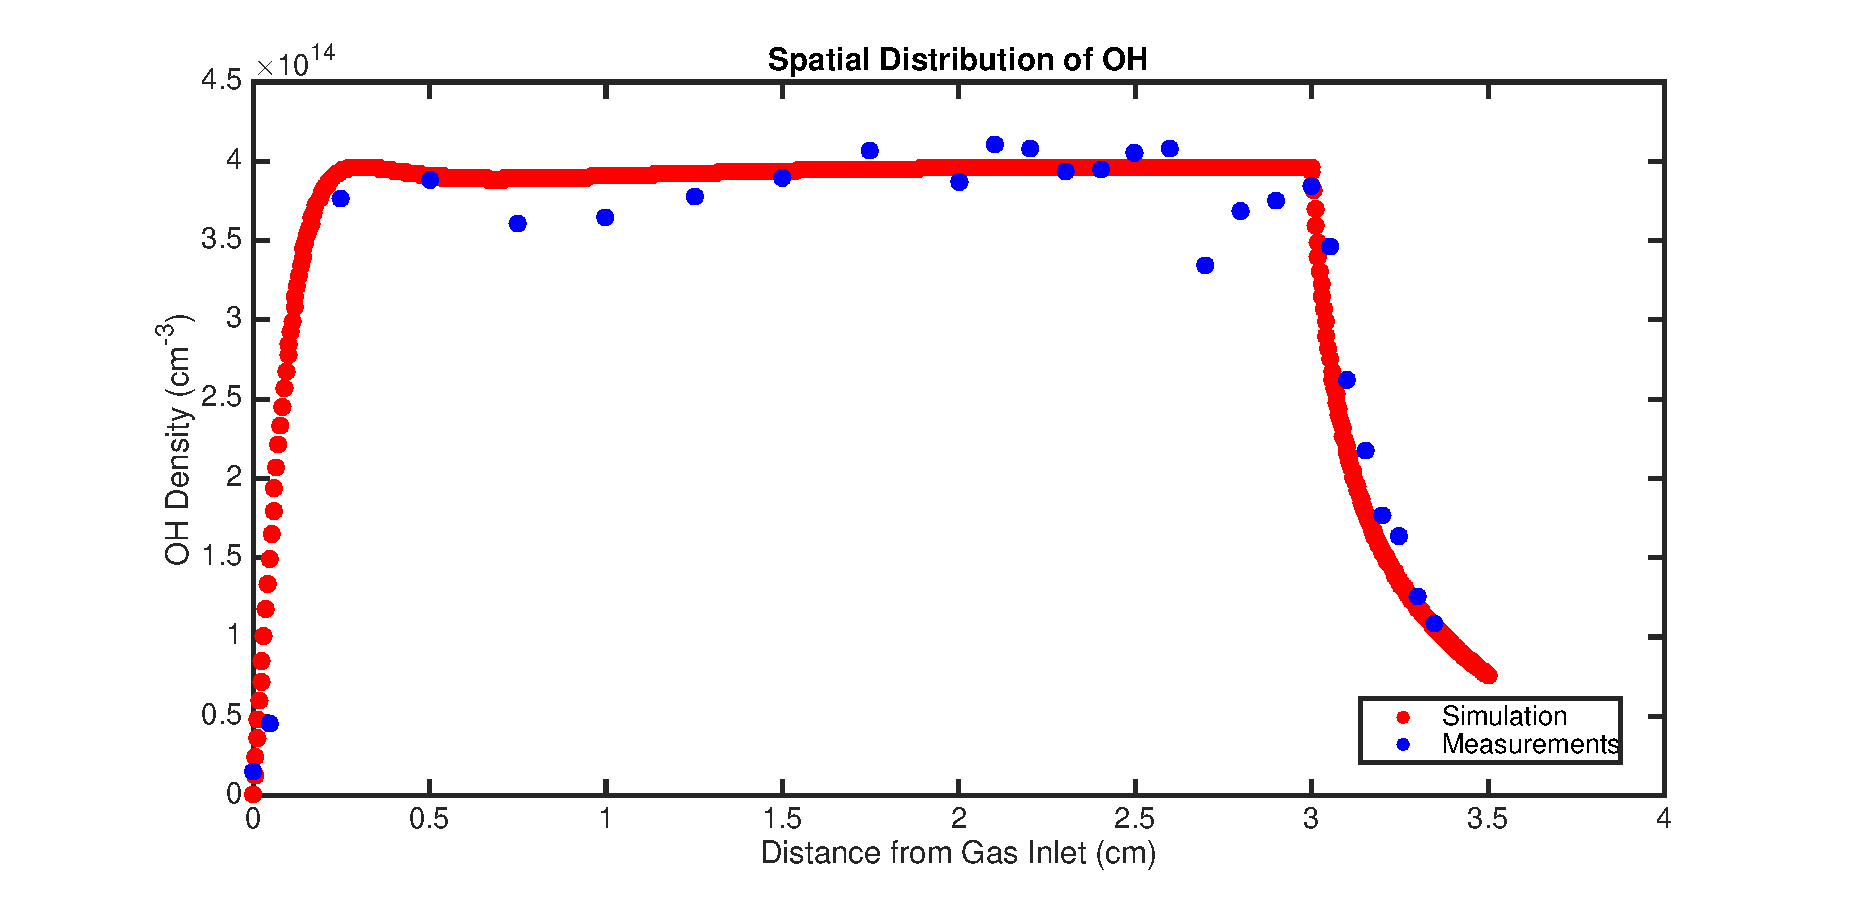
\includegraphics[width=\textwidth]{Figures/SpatialGraph}
\caption{
Figure showing OH density, from experiment and simulation, as a function of distance along the plasma channel from the gas inlet. Absorption spectroscopy was performed at 0.5 - 1 mm intervals along the 30 mm length of the electrodes (0-3 cm), plus at 0.5 mm intervals beyond the end of the plasma region (3.05-3.35 mm). The position along the plasma channel in cm is shown on the x axis, and the corresponding OH density is shown in cm\textsuperscript{-3} on the y axis. The plasma was operated at 5.39 W (16.33 W/cm\textsuperscript{3}) with a feed gas flow rate of 5 slm helium with 5400 ppm water. 
The simulation was carried out at the same plasma parameters.
Blue points denote experimental data, red points show simulated data.}
\label{SpatialGraph}
\end{figure}

As shown in figure \ref{SpatialGraph}, there is very good agreement both in trend and absolute densities between both the simulated and measured data.

\subsection{Power Variation}

Secondly, the effect of power variation on OH density in the plasma was investigated.
For this the power applied was varied in the range of 2.99 - 5.39 W, and absorption spectroscopy measurements were taken at 2 cm from the gas inlet.
Similarly, the simulations were done at the same powers and data points taken at the same position.
Comparison between measurements and simulations are shown in figure \ref{PowerVariation}.

As shown in figure \ref{PowerVariation}, the simulated OH density is lower that the average measured density, however, it is generally within the range of measurements, suggesting it is within the error range of the measurements.

\begin{figure}
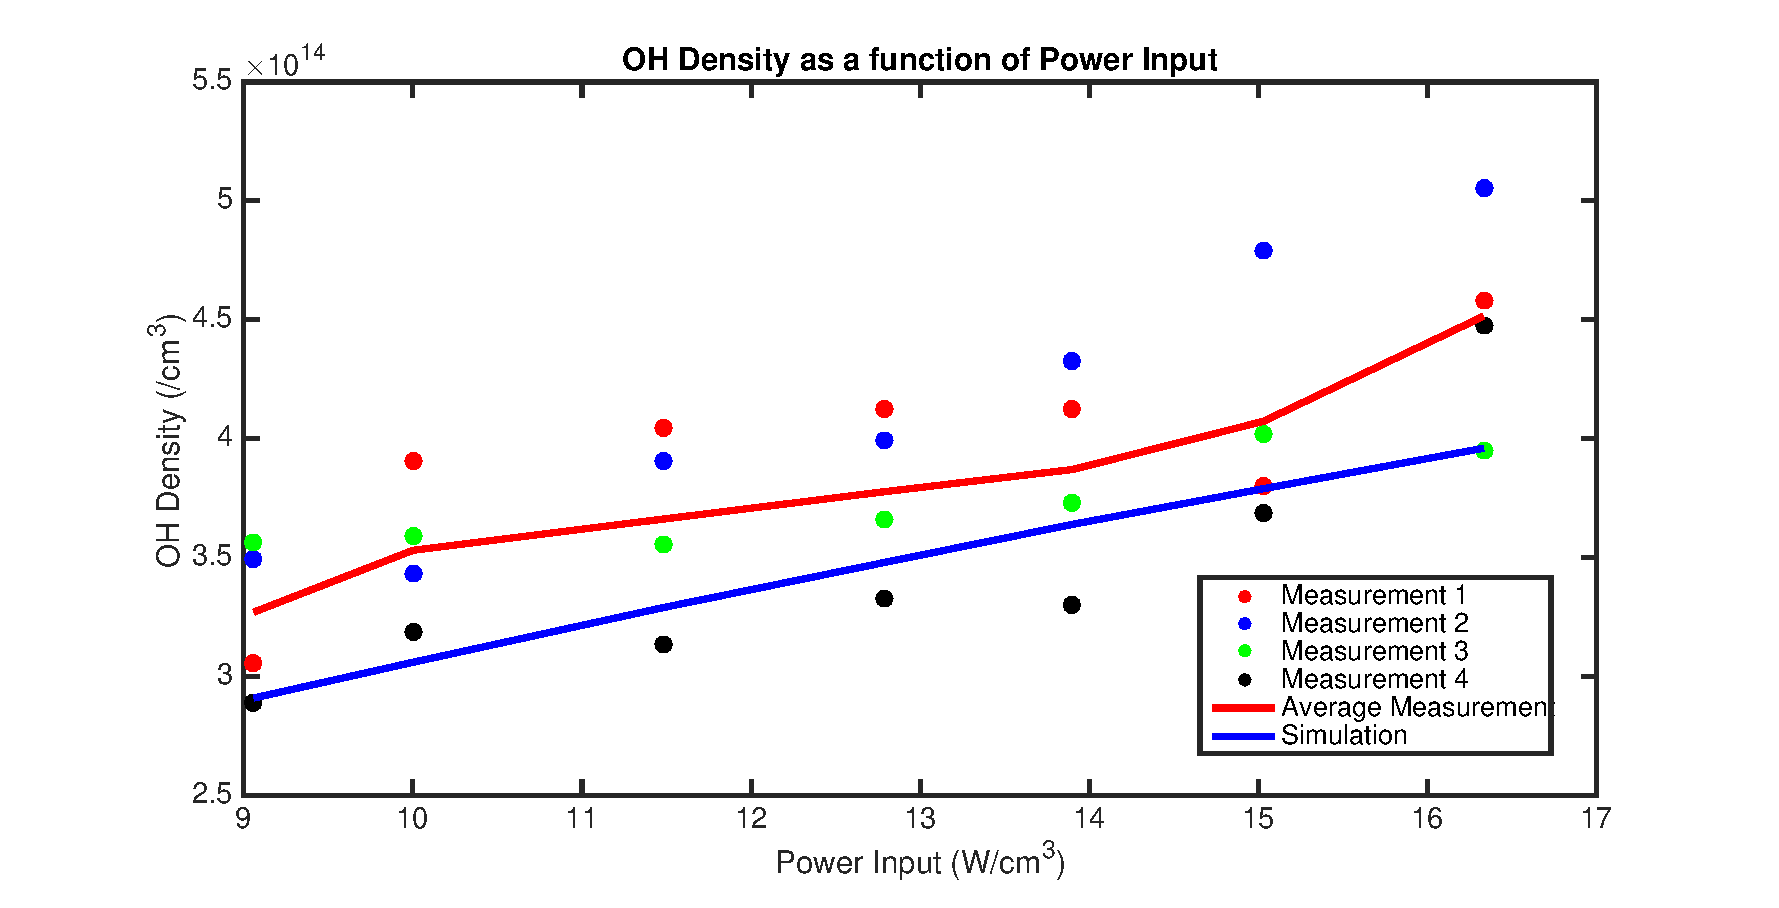
\includegraphics[width=\textwidth]{Figures/PowerVariation}
\caption{Figure showing OH density as a function of plasma power. Absorption spectroscopy was performed at a point 20mm from the gas inlet while power being dissipated in the plasma was varied within the range of 9.06 - 16.33 W cm\textsuperscript{-3} (2.99 - 5.39 W), as shown on the x axis. Total gas flow to the plasma was kept constant at 5 slm helium with $\sim$5400 ppm water. The experiment was repeated four times, each repeat is shown in red, blue, green and black points. The average measured density is shown by the red line.
Simulation using GlobalKin is shown by the blue line, using the same plasma parameters as the experiment, and simulated data taken at the same point in the plasma channel.
The OH density is shown on the y axis in cm\textsuperscript{-3}, and the power density input is shown on the x axis in W/cm\textsuperscript{3}.}
\label{PowerVariation}
\end{figure}


\subsection{Next Steps: Development of Air Plasma Model}

The next stage of my project is to model air plasmas, as these are the focus of my work.
A collaboration was recently started across many plasma groups in Europe, with the aim of different models and chemistry sets for air plasmas.
This is of interest in my project as it will allow me to develop and benchmark an air plasma model to other simulations and chemistry sets.

When modelling plasmas, it is important to note that there are two main considerations.
Firstly, the model platform to use, for example GlobalKin, and secondly, the reaction chemistry set.
The idea for the collaboration is that each research group uses their own plasma model and chemistry set, then specific outputs from each group can be anonymised and distributed through the entire consortium for comparison.
Following this, there can be iterations of the process until groups are happy with their simulations/outputs.
The collaboration will be run in a series of stages.
Firstly, codes will all be initialised, using parameters and short reaction sets provided by the coordinator, so that outcomes can be compared and groups can check that their codes are appropriate for the task.
At this point, we need to make sure that GlobalKin is a suitable model for carrying out the simulations in line with the specified inputs in order to give the correct outputs.
The deadline for this stage is currently 20.1.17.
Following this, the simulations of air plasmas can begin.

As part of this collaboration I am investigating air reaction chemistry sets that have been used before for air plasma modelling to help decide on which reaction set we will use, and I will be carrying out simulations.


%\section*{Modelling Air Plasmas}
%\subsection*{What's been done before?} 
%There are many different models and chemistry sets that have been used for previous attempts at modelling air plasmas. 
%Issues with modelling atmospheric pressure air plasmas is the number of species that are involved and the high collisionality environment.
\subsection{Chemistry Reaction Sets}
For the purposes of both the collaboration, and my own research project, the aim is to find an appropriate air chemistry reaction set that can be used for modelling.

Firstly, in the original thesis and subsequent publication presenting the GlobalKin code, there is a full reaction chemistry set presented for modelling humid air plasmas interacting with polypropylene surfaces \cite{Dorai2002modeling, Dorai2003a}.
Here, they consider two sets.
Firstly the gas phase (consisting of species formed from, and reactions involving the flow gas containing N$_2$/O$_2$/H$_2$O in 79/20/1 proportions), and secondly the surface interaction chemistry. 
For the purposes of our model, only the gas phase reactions are of interest.
The gas phase consists $\sim$334 reactions and 56 species. 
The model used is GlobalKin and, therefore, works as outlined above.

However, there are other types of models that have been used for modelling air plasmas.
For example, in a recent paper by Kutasi \textit{et al} \cite{Kutasi2016tuning} they present a model for an Ar/N$_2$/O$_2$ plasmas.
Their main aim is to investigate the afterglow region of a plasma, both using Ar/N$_2$/O$_2$ mixture and using just N$_2$/O$_2$.
The model presented has a Boltzmann equation solver, which calculates the EEDF by taking into account electron impact with the parent gas, major species produced by plasma, and other electrons.
For heavy species, zero dimensional continuity equations are constructed and the electric field is calculated self-consistently by satisfying the property of quasineutrality, ie, the electrons lost must equal the electrons produced.
The model also incorporates a chemistry set and is run either using the ternary Ar/N$_2$/O$_2$ mixture, or the binary N$_2$/O$_2$ mixture.
Unfortunately, the full reaction set is not presented and the paper states that the full reaction set will be presented in detail elsewhere.
However, the N$_2$-O$_2$ reactions are taken mainly from \cite{Guerra1997self, Pintassilgo2005modelling, Kutasi2008modelling}.
These papers present models with aims of further understanding dynamics of species production in low pressure N$_2$O$_2$ glow-discharges \cite{Guerra1997self} and production of species important for sterilisation processes, in particular for the emission of specific wavelength UV radiation \cite{Pintassilgo2005modelling, Kutasi2008modelling}.
These models include not only ground and excited states of particles, but also often take into account the distribution of vibrational states of molecules, which may, or may not, be important for our modelling.


%These papers presented models for:
%\begin{itemize}
%\item Guerra \textit{et al} \cite{Guerra1997self} - "low pressure N$_2$O$_2$ glow discharge. Importance for studying for plasma reactors for chemical synthesis, depollution of atmosphere and surface treatments. Study of non equilibrium coupling between the electron and heavy particle kinetics. Done by solving Boltzmann equation and rate balance equations for certain atoms and vibrational states of molecules. Improved on the previous model \cite{Guerra1995non}. Self-consistent maintenance reduced electric field calculated.
%\item Pintassilgo \textit{et al} \cite{Pintassilgo2005modelling} - Model for helping to understand the dynamics of particular NO and O species (as these are relevant for sterilisation purposes, in particular their emission of specific UV radiation). The model starts by calculating EEDF and the vibrational distribution functions of certain molecules and initial concentrations of other species. 
%"kinetic model for looking at increasing sterilising species (specific NO and O species).
%\item Kutasi \textit{et al} \cite{Kutasi2008modelling} - 
%\end{itemize}
%
%In 1997, Guerra \textit{et al} \cite{Guerra1997self} presented a paper (as an extension to a previous publication \cite{Guerra1995non}), whereby 


%is a paper building on a previous one \cite{Guerra1995non}, where some vibrational states of N$_2$ had to be an input parameter of the model, taken from experimental data. Here, the model consists of the electron Boltzmann equation coupled to rate balance equations for vibrationally excited molecules of N$_2$ and O$_2$, electronically excited states of N$_2$ and NO, N and O species (with term symbols attached?). All this plus continuity equations for electrons and main positive ions (N$_2^+$, N$_4^+$, O$^+$, O$_2^+$, NO$^+$). TO DO - read this paper to find out the point of what it was doing. What was the model doing? 
%\cite{Pintassilgo2005modelling} is looking at sterilisation processes and therefore using a model to predict ways of maximising concentrations of NO ($B ^2\Sigma$) and O($^3P$). 
%The model starts by working out the EEDF and also the vibrational distribution function of some molecules. 
%It also calculates the concentrations of N$_2$ and O$_2$ electronic states, N and O atoms, NO, NO$_2$ and O$_3$ species, as well as the positive and negative ions formed in the discharge. However, not sure what the type of model is because very few reactions shown...
%\cite{Kutasi2008modelling} is a paper about a 3-D hydrodynamic model, with regards to UV emission from the plasma, to be used for sterilisation.
%
%However, whilst they do not cite their entire reaction chemistry, they do provide references for reactions involving the different gases. Of particular interest are the references relating to reactions involving N$_2$ and O$_2$.
%
%There are lots of chemistry sets that have been used before for air plasma modelling.
%Spacecraft re-entry? 
%\begin{itemize}
%\item Lazarou2016numerical - He/Air plasma. Investigating the effect of air in He plasmas and therefore the effects of impurities on the running of He plasmas. 27 species, 153 reactions. No NO$_x$ species included as increased computational time too much without affecting simulation results significantly \cite{Lazarou2016numerical}.
%\item Murakami2014afterglow -  This is modelling air impurities in He/O$_2$ plasmas too. Very small percentage air mixture ($\approx$ 0.025\%). The importance of the air in the model was to see how different percentages of air impurities in the He plasma affected the densities of different plasma species.\cite{Murakami2014afterglow}
%\item here is another paper \cite{Gordiets1995kinetic}.
%\item Rate constants for reactions in global chemistry models affect species density evolution over time. 
%By evaluating the reactions/rate constants which contribute the most to a He/O$_2$ plasma chemistry, the comprehensive reaction scheme (25 species, 373 reactions \cite{Turner2015uncertainty}) was rationalised to a reduced scheme (12 species, 51 reactions). The initial rate constants determined through experimentation/theory have an associated error with them. Therefore, the study also looked at which rate constants for each of the included reactions contributed the most error to the system. It was found that it was a small proportion of the reaction rate constants that were responsible for the majority of the error. In particular, rate constants for 3 body reactions involving He and electron reactions with O species, had the highest contribution to the overall error \cite{Turner2016uncertainty}.
%\item A collisional radiative model (looking at the distribution of atoms/molecules over their excited states \cite{Sijde1984collisional}) was developed to look at air plasmas formed during spacecraft entry to upper levels of a planets atmosphere. This isn't really what I'm looking for though as it is too much to do with different vibrationally excited states... I think \cite{Bultel2006collisional}.
%\item Really useful paper that used GlobalKin for argon plasma going into humid air, but also has good intro on some air plasma chemistry sets \cite{Gaens2013kinetic}.
%\item This paper talks about modelling surface microdischarges. Ie from top to bottom: driven electrode, dielectric, discharge, grounded mesh, effluent, surface to be treated. 53 species, 624 reactions \cite{Sakiyama2012plasma}.
%\item Kutasi \cite{Kutasi2016tuning}(Vasco paper) does not cite it's full chemistry set for Ar/O$_2$/N$_2$. However, it says it's set it based mainly on other papers. Of particular interest it's N$_2$/O$_2$ interactions come mainly from \cite{Pintassilgo2005modelling, Guerra1997self, Kutasi2008modelling}.
%\item \cite{Guerra1997self} is a paper building on a previous one \cite{Guerra1995non}, where some vibrational states of N$_2$ had to be an input parameter of the model, taken from experimental data. Here, the model consists of the electron Boltzmann equation coupled to rate balance equations for vibrationally excited molecules of N$_2$ and O$_2$, electronically excited states of N$_2$ and NO, N and O species (with term symbols attached?). All this plus continuity equations for electrons and main positive ions (N$_2^+$, N$_4^+$, O$^+$, O$_2^+$, NO$^+$). TO DO - read this paper to find out the point of what it was doing. What was the model doing? 
%\item \cite{Pintassilgo2005modelling} is looking at sterilisation processes and therefore using a model to predict ways of maximising concentrations of NO ($B ^2\Sigma$) and O($^3P$). 
%The model starts by working out the EEDF and also the vibrational distribution function of some molecules. 
%It also calculates the concentrations of N$_2$ and O$_2$ electronic states, N and O atoms, NO, NO$_2$ and O$_3$ species, as well as the positive and negative ions formed in the discharge. However, not sure what the type of model is because very few reactions shown...
%\item \cite{Kutasi2008modelling} is a paper about a 3-D hydrodynamic model, with regards to UV emission from the plasma, to be used for sterilisation.
%
%\item \cite{Dorai2002modeling} is a thesis from the Kushner group who designed GlobalKin. 
%In this, a full reaction set is listed for humid air interaction with polypropylene surfaces.
%It says there are 90 species and nearly 400 reactions included in the set (56 species containing only N, O and H. Lots of reactions).
%
%
%\end{itemize}
%
%\section{Electron orbitals, angular momentum and spin}
%Understanding term symbols:
%\begin{equation}
%^{2S+1}L_{J}
%\end{equation}
%where $S$ is the total spin quantum number, $L$ is the orbital quantum number (i.e. S, P, D, F etc), and $J$ is the total angular momentum quantum number.
%$S$ is related to the number of unpaired electrons present in the outermost electron shell.
%Each electron $S = \pm \frac{1}{2}$, therefore, by adding up the spin of every electron, this gives the overall spin. If there are no unpaired electrons, $S = 0$. However, if there is one, spin-up free electron, $S = +\frac{1}{2}$ etc. 
%The term $2S + 1$ gives the multiplicity of the atom/molecule ($2S + 1 = 1 \rightarrow singlet, 2 \rightarrow doublet$ etc)
%Therefore, for the above atom where $S = +\frac{1}{2}$, $2S + 1 = 2$, making it a doublet.
%L is given by the type of outer shell, i.e. S, P, D, F etc orbital.
%
%
%\section{Experimental}
%\subsection{What's been done}
%Nothing
%\subsection{What are the next steps}
%Aim to measure NO? And see what happens to cells when treated with the plasma?!
%Combine what we see with model... May be He/Air (He/O$_2$/N$_2$) gas mixture.
%

\bibliographystyle{ieeetr}
\bibliography{/Users/hld523/Bibliography/MyPapers}
\end{document}  